\documentclass[a4paper,12pt]{article}
\usepackage[top = 2.5cm, bottom = 2.5cm, left = 2.5cm, right = 2.5cm]{geometry}
\usepackage[T1]{fontenc}
\usepackage[utf8]{inputenc}
\usepackage{multirow} 
\usepackage{booktabs} 
\usepackage{graphics}
\usepackage{graphicx}
\usepackage{subcaption}
\usepackage{mwe}
\usepackage[spanish]{babel}
\usepackage{setspace}
\setlength{\parindent}{0in}
\usepackage{float}
\usepackage{fancyhdr}
\usepackage{amsmath}
\usepackage{amssymb}
\usepackage{amsthm}
\usepackage{natbib}
\usepackage{graphicx}
\usepackage{subcaption}
\usepackage{booktabs}
\usepackage{etoolbox}
\usepackage{apalike}
\usepackage{minibox}
\usepackage{hyperref}
\usepackage{xcolor}
\usepackage{tcolorbox}
\AtBeginEnvironment{align}{\setcounter{equation}{0}}
\newenvironment{solution}
  {\renewcommand\qedsymbol{$\square$}\begin{proof}[\textcolor{blue}{Solución}]}
  {\end{proof}}

\pagestyle{fancy}

\fancyhf{}

\lhead{\footnotesize Algoritmos y Estructuras de Datos}
\rhead{\footnotesize  Rudik Roberto Rompich}
\cfoot{\footnotesize \thepage}

\begin{document}
    \thispagestyle{empty} 
    \begin{tabular}{p{15.5cm}}
    \begin{tabbing}
    \textbf{Universidad del Valle de Guatemala} \\
    Departamento de Matemática\\
    Licenciatura en Matemática Aplicada\\\\
   \textbf{Estudiante:} Rudik Roberto Rompich\\
   \textbf{E-mail:} \textcolor{blue}{ \href{mailto:rom19857@uvg.edu.gt}{rom19857@uvg.edu.gt}}\\
   \textbf{Carné:} 19857
    \end{tabbing}
    \begin{center}
        CC2003 - Algoritmos y Estructuras de Datos - Catedrático: Melvin García\\
        \today
    \end{center}\\
    \hline
    \\
    \end{tabular} 
    \vspace*{0.3cm} 
    \begin{center} 
    {\Large \bf Proyecto 2 - Sistema de recomendaciones 
} 
        \vspace{2mm}
    \end{center}
    \vspace{0.4cm}
%---------------------------
%\begin{tcolorbox}[colback=gray!15,colframe=black!1!black,title=A nice heading]
%\end{tcolorbox}

%\fbox{lol}
%---------------------------

\section{Investigación}

Los algoritmos descritos a continuación son tomados del libro de \cite{needham2019graph}. 

\subsection{Strongly Connected Components}

El SCC hace referencia a un algoritmo que encuentra conjuntos de nodos conectados en grafos directos; donde cada nodo es alcanzable en ambas direcciones desde cualquier otro nodo del mismo conjunto. 

\begin{center}
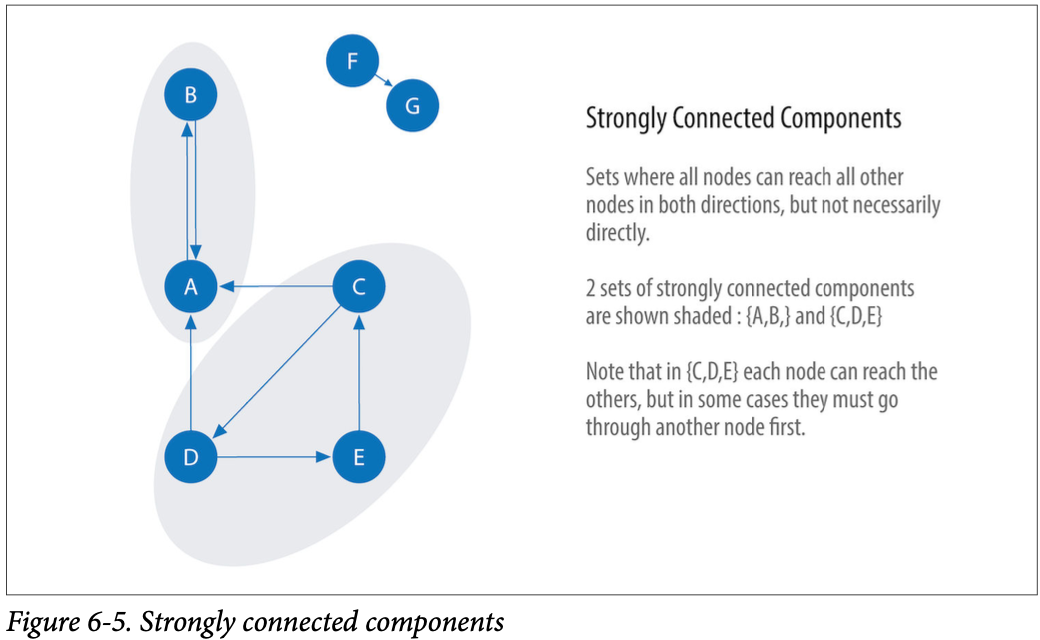
\includegraphics[scale=0.4]{Images/1-SCC.png}    
\end{center}

Características: 

\begin{itemize}
    \item No es necesario que los nodos sean vecinos, pero deben haber aristas entre todos los nodos del conjunto. 
    \item Descomponer un grafo directo en un algoritmo SCC es una aplicación de otro algoritmo: \textit{Depth First Search algorithm}.  
    \item Un componente fuertemente conectado tiene una utilidad directa o inclinación para encontrar comportamientos similares. 
\end{itemize}

\subsection{Betweenness Centrality}

Este es un algoritmo que tiene como propósito detectar la cantidad de influencia que un nodo tiene sobre un flujo de información o recursos de un grafo. Una analogía sería: un algoritmo que intenta encontrar nodos que sirvan como puentes de una parte del grafo hacia otra. 

Características: 

\begin{itemize}
    \item Este algoritmo primero calcula la trayectoria más corta (\textit{weighted}) entre cada par de nodos en un grafo conectado. Cada nodo recibe un puntaje, basado en el número de trayectorias que pasan a través del nodo. Entre más trayectorias cortas pase un nodo, más alto es su puntaje.
    \item Puentes y puntos de control 
    \begin{itemize}
        \item[Puente:] Puede ser un nodo o una relación. Se pueden identificar, ya que si si se remueve un punte, el grafo se convierte en un grafo disconexo. 
        \item[Pivote:] Un nodo es considerado pivote para otros dos nodos, si ese nodo está en la trayectoria más corta de esos dos nodos. Es decir: 
        \begin{center}
            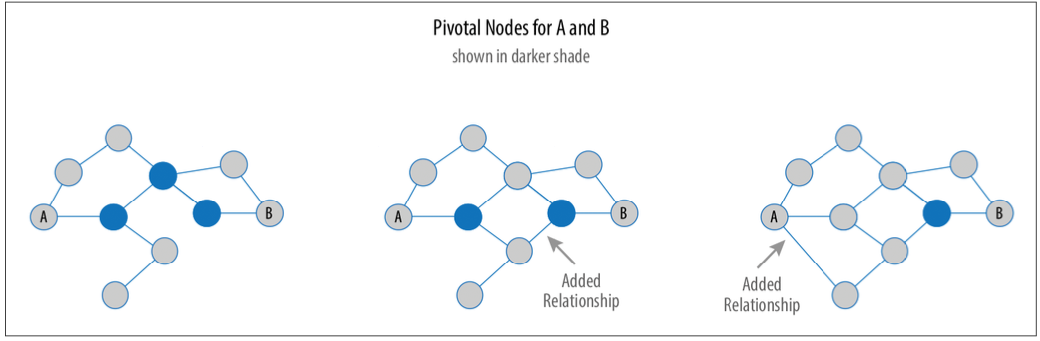
\includegraphics[scale=0.4]{Images/1-pivotal.png}
        \end{center}
    \end{itemize}
\end{itemize}
\subsubsection{¿Cómo se calcula el betweenness centrality?}

$$B(u)=\sum_{s\neq u\neq t}\frac{p(u)}{p}$$
En donde: 
\begin{enumerate}
    \item $u$ es un nodo. 
    \item $p$ es el número de trayectorias cortas entre los nodos $s$ y $t$.
    \item $p(u)$ es el número de trayectorias cortas entre los nodos $s$ y $t$ que pasan a través del nodo $u$. 
\end{enumerate}

\begin{center}
    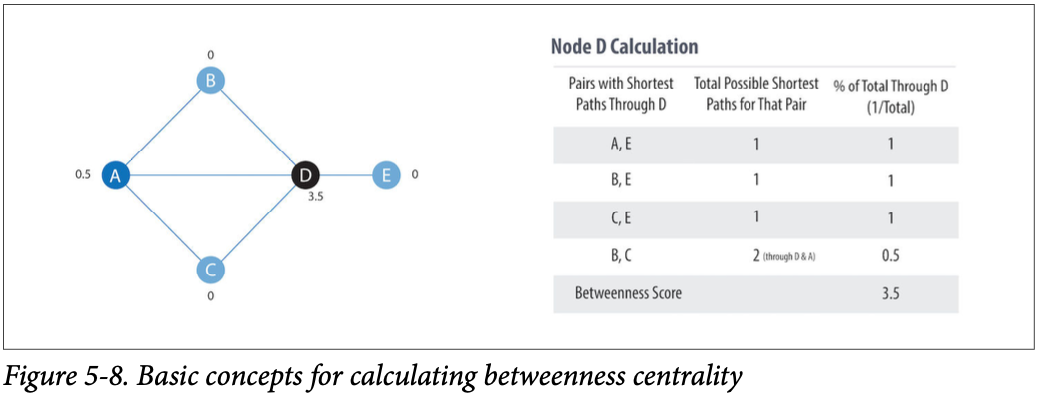
\includegraphics[scale=0.4]{Images/1-bc.png}
\end{center}

Un ejemplo: 

\begin{center}
    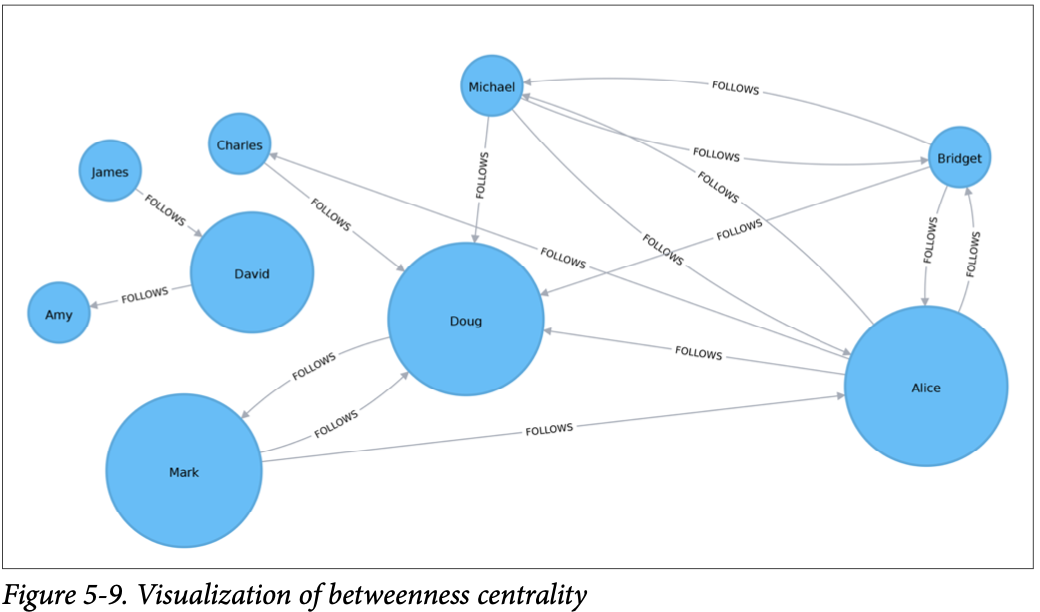
\includegraphics[scale=0.4]{Images/1-bc2.png}
\end{center}

\subsection{PageRank}
PageRank es el mejor algoritmo de centralidad conocido. El algoritmo mide la transitividad (o dirección) de la infuencia de los nodos. PageRank 
considera la influencia de los vecinos de un nodo y de sus vecinos. Por ejemplo, una analogía, una persona que tenga pocos amigos poderosos puede ser más influyente que alguien que tenga muchos amigos pero menos poderosos. 

\subsubsection{¿Cómo se calcula?}
Citando literalmente a \cite{needham2019graph}. «PageRank is defined in the original Google paper as follows: 
$$PR(U)=(1-d)+d\left(\frac{PR(T_1)}{C(T_1)}+\cdots +\frac{PR(T_n)}{C(T_n)}\right)$$
where: 

\begin{enumerate}
    \item  We assume that a page u has citations from pages $T_1$ to $T_n$.
    \item $d$ is a damping factor which is set between 0 and 1. It is usually set to 0.85. You can think of this as the probability that a user will continue clicking. This helps minimize rank sink, explained in the next section.
    \item $1-d$ is the probability that a node is reached directly without following any rela‐ tionships.
    \item $C(T_n)$ is defined as the out-degree of a node $T$.»
\end{enumerate}
\begin{center}
    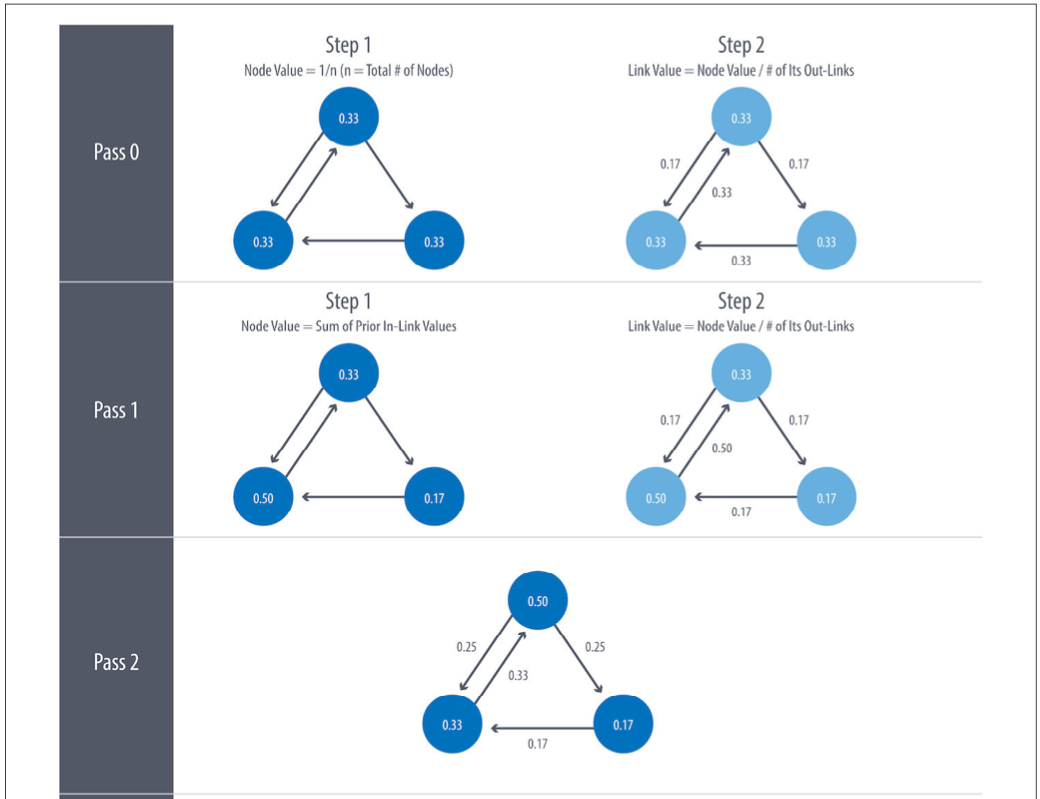
\includegraphics[scale=0.35]{Images/1-pr1.png}
    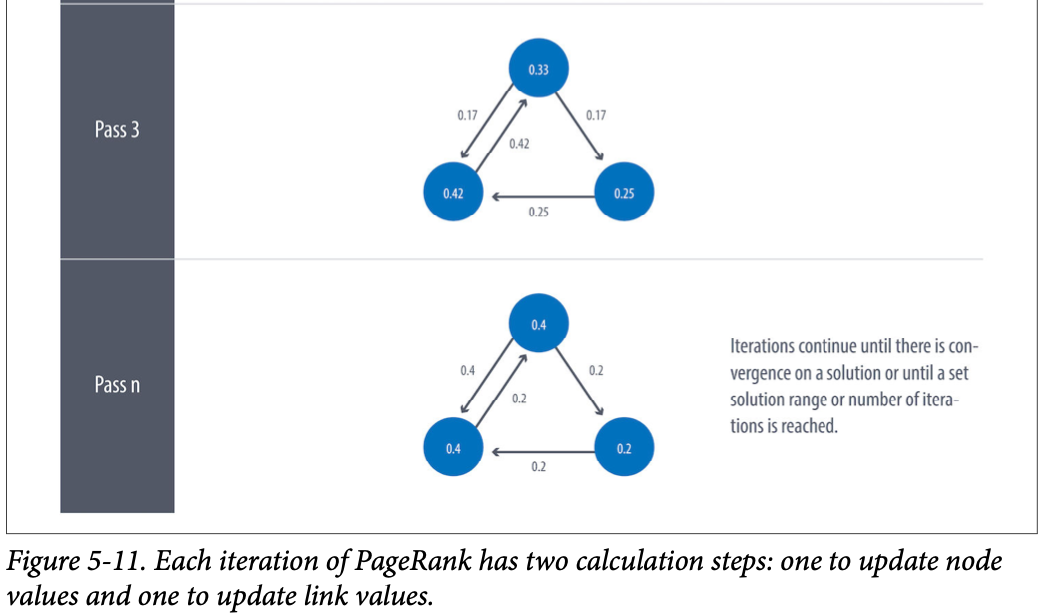
\includegraphics[scale=0.35]{Images/1-pr2.png}
\end{center}
\section{Design Thinking}
\subsection{Empatía}

Cada semestre en el Club de Ajedrez de la Universidad del Valle de Guatemala, entran decenas de personas esperando inmiscuirse en el mundo del ajedrez; sin embargo, se encuentran con la barrera del desconocimiento de varios principios fundamentales de este deporte y finalmente, estas personas, terminan abandonando el club o simplemente siendo miembros inactivos. \newline\newline
La junta directiva del Club de Ajedrez ha intentando implementar diversas actividades para evitar que los miembros se vuelven inactivos; por lo cual, se busca generar un sistema de recomendaciones que ayude a los miembros del club a tener una visión más amplia del ajedrez y que este se vuelva más envolvente en sus vidas.

\subsection{Definición}
Los principales problemas identificados son: 
\begin{enumerate}
    \item Desconocimiento de las fases del ajedrez. 
    \item Desconocimiento de las estrategias adecuadas para cada nivel de juego. 
    \item Herramientas adecuadas para aprender a jugar ajedrez.
\end{enumerate}

El problema propuesto a resolver es un sistema de recomendaciones de cierto de tipo de posiciones. 

\subsection{Ideación}
Existen diversas fases en el ajedrez, sin embargo, el sistema de recomendaciones se centrará en la primera fase: la apertura. 

El propósito es encontrar las aperturas jugadas por los miembros de club que tengan el mismo nivel. Es decir, las 3 categorías: 
\begin{enumerate}
    \item Principiante 
    \item Intermedio 
    \item Avanzado 
\end{enumerate}
\subsection{Prototipos}
La primera fase se ha basado en elegir los parámetros más idóneos a evaluar, se han propuesto los más relevantes: 

\begin{enumerate}
    \item Plataforma favorita para jugar. 
    \item Plataforma con los mejores recursos para aprender. 
    \item Modalidad favoritas de juego. 
    \item Modalidad que le gusta observar en Youtube, Twitch, etc... 
    \item Parte favorita de una partida. 
    \item Su nivel de juego en Blitz.
    \item Su nivel de juego en Rápidas.
    \item Apertura que juega.
    \item Defensa que juega.
\end{enumerate}

De los cuales, únicamente se tomaron en cuenta los siguientes parámetros: 

\begin{enumerate}
    \item $PLATAFORMA$ - Plataforma favorita para jugar. 
    \item $APERTURA$ - Apertura que juega.
    \item $DEFENSA$ - Defensa que juega.
    \item $PARTE\_ FAVORITA$ - Parte favorita de una partida. 
    \item $NIVEL\_BLITZ$ - Su nivel de juego en Blitz.
    \item $NIVEL\_RAPIDAS$ - Su nivel de juego en Rápidas. 
\end{enumerate}
\subsection{Testing}
La encuesta se encuentra aquí: \textcolor{blue}{\href{https://forms.gle/5swmk2VsKMPd1hha6}{https://forms.gle/5swmk2VsKMPd1hha6}}.\newline\newline
La encuesta se basó en las siguientes preguntas: 
\begin{enumerate}
    \item Nivel de juego en blitz  (\textit{Considere un estimado de su rating en chess.com: (1) Principiante [0 a 1400 elo], (2) Intermedio [1400 - 1600 elo], (3) Avanzado [1600- infinito].}): 
    \begin{enumerate}
        \item Principiante 
        \item Intermedio 
        \item Avanzado
    \end{enumerate}
    \item Nivel de juego en rápidas (\textit{Considere un estimado de su rating en chess.com: (1) Principiante [0 a 1400 elo], (2) Intermedio [1400 - 1600 elo], (3) Avanzado [1600- infinito].}): 
    \begin{enumerate}
        \item Principiante 
        \item Intermedio 
        \item Avanzado
    \end{enumerate}
    \item ¿Cuál es tu parte favorita del ajedrez?
    \begin{enumerate}
        \item Apertura 
        \item Intermedio 
        \item Final
    \end{enumerate}
    \item ¿Cuál es tu plataforma favorita para jugar?
    \begin{enumerate}
        \item Lichess.org
        \item Chess.com
        \item Chess24.com
        \item Otro
    \end{enumerate}
    \item De las aperturas anteriores, ¿cuál se adecúa más a tu estilo de juego? 
    \begin{enumerate}
        \item Italiana/Española
        \item Inglesa
        \item Sistema Londres
        \item Fianchetto
    \end{enumerate}
    \item De las defensas anteriores, ¿cuál se adecúa más a tu estilo de juego? 
    \begin{enumerate}
        \item Eslava
        \item Francesa
        \item Caro-Kann
        \item Siciliana
    \end{enumerate}
\end{enumerate}
\subsubsection{Explicación}

Por el planteamiento del problema, la idea es que el usuario ingrese su nivel de juego (principiante, intermedio o avanzado). Entonces el programa le recomendará la plataforma, apertura y defensa de jugadores de su mismo nivel. Desde el punto de vista matemático, el programa únicamente buscará las relaciones y nodos conectados a los niveles de juego. \newline

Las aperturas y defensas en las siguientes páginas. 
\newpage 
\begin{figure*}[ht]
        \centering
        \begin{subfigure}[b]{0.475\textwidth}
            \centering
            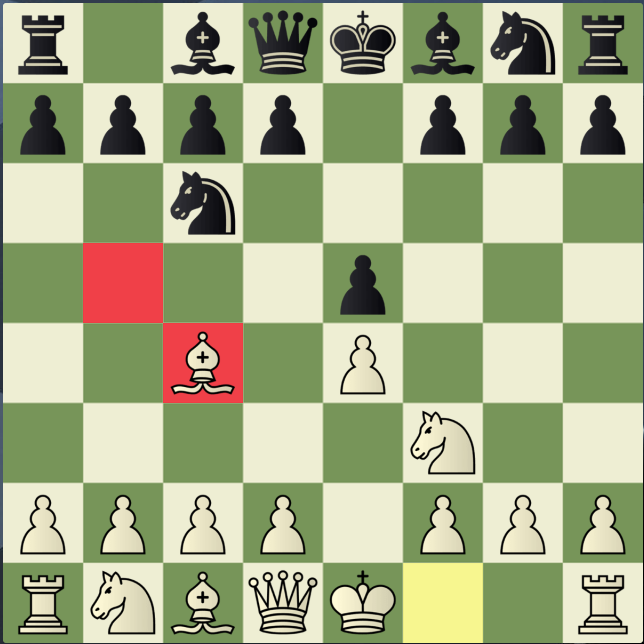
\includegraphics[width=\textwidth]{Images/Design/a-1.png}
            \caption{Italiana/Española} 
        \end{subfigure}
        \hfill
        \begin{subfigure}[b]{0.475\textwidth}  
            \centering 
            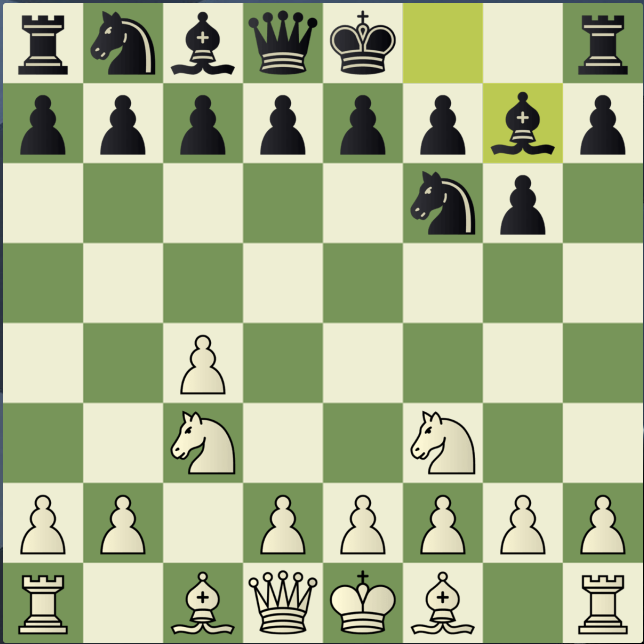
\includegraphics[width=\textwidth]{Images/Design/a-2.png}
            \caption{Inglesa}
        \end{subfigure}
        \vskip\baselineskip
        \begin{subfigure}[b]{0.475\textwidth}   
            \centering 
            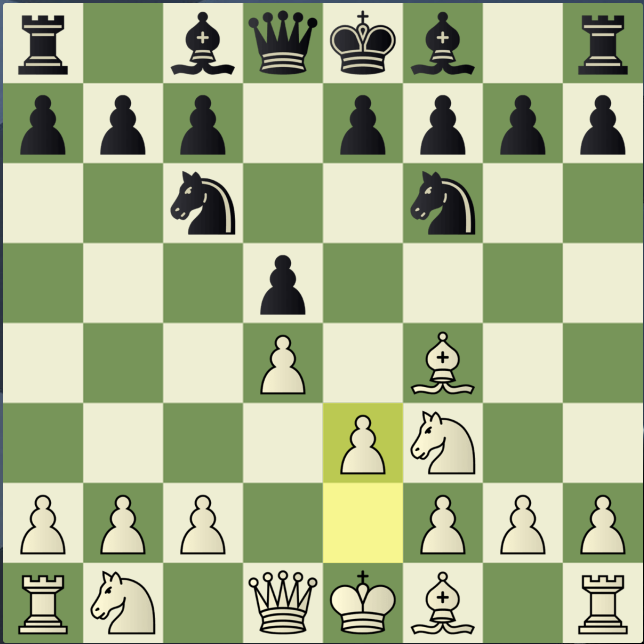
\includegraphics[width=\textwidth]{Images/Design/a-3.png}
            \caption{Sistema Londres}  
        \end{subfigure}
        \hfill
        \begin{subfigure}[b]{0.475\textwidth}   
            \centering 
            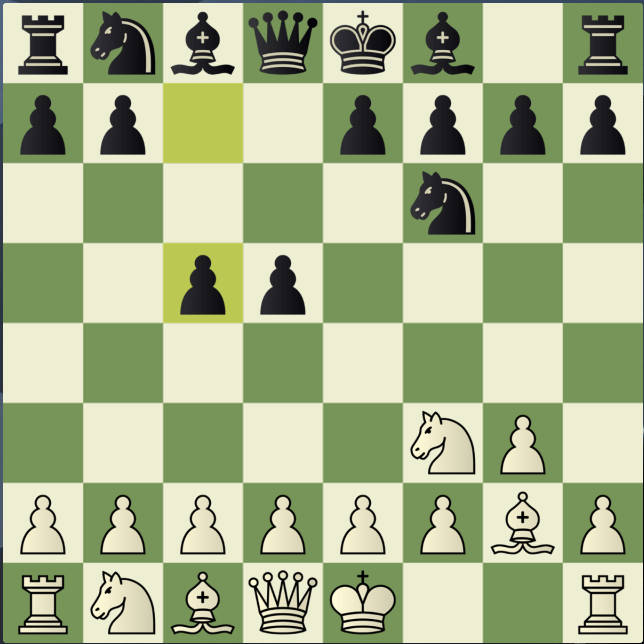
\includegraphics[width=\textwidth]{Images/Design/a-4.png}
            \caption{Fianchetto}  
        \end{subfigure}
        \caption{Aperturas comunes en ajedrez.}
    \end{figure*}
    \newpage 
\begin{figure*}[ht]
        \centering
        \begin{subfigure}[b]{0.475\textwidth}
            \centering
            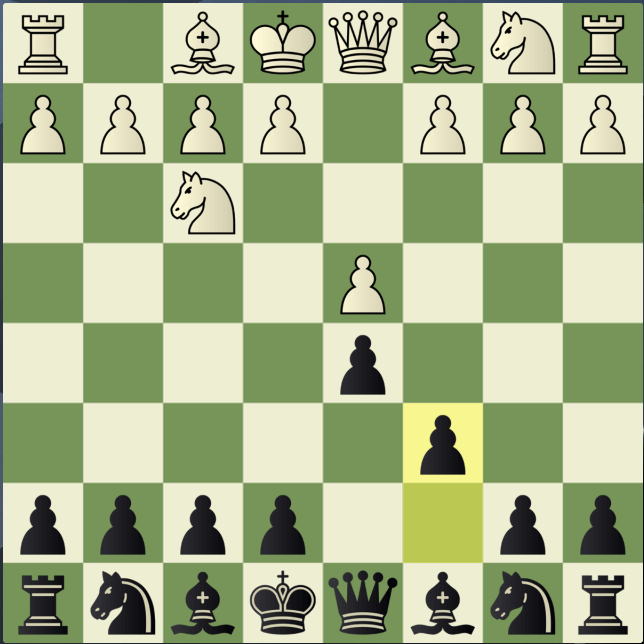
\includegraphics[width=\textwidth]{Images/Design/d-1.png}
            \caption{Eslava}
        \end{subfigure}
        \hfill
        \begin{subfigure}[b]{0.475\textwidth}  
            \centering 
            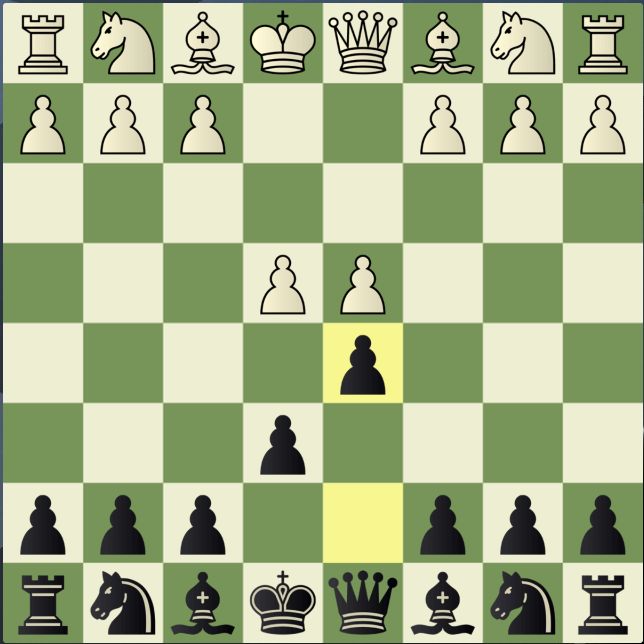
\includegraphics[width=\textwidth]{Images/Design/d-2.png}
            \caption{Francesa}
        \end{subfigure}
        \vskip\baselineskip
        \begin{subfigure}[b]{0.475\textwidth}   
            \centering 
            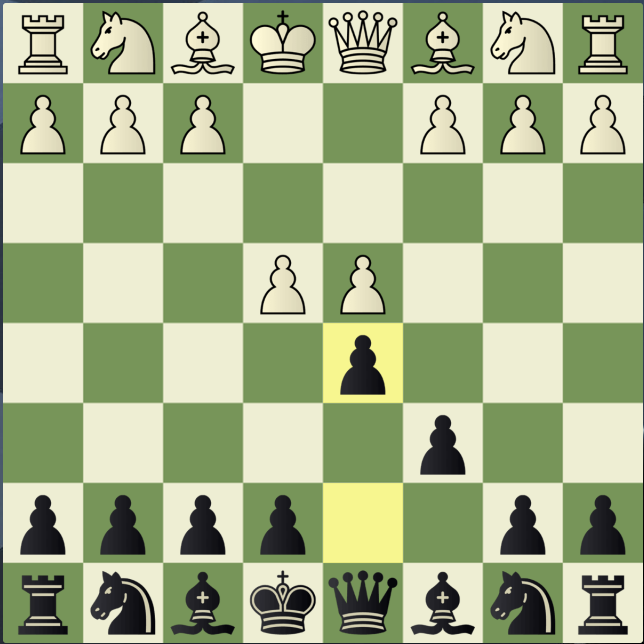
\includegraphics[width=\textwidth]{Images/Design/d-3.png}
            \caption{Caro-Kann}
        \end{subfigure}
        \hfill
        \begin{subfigure}[b]{0.475\textwidth}   
            \centering 
            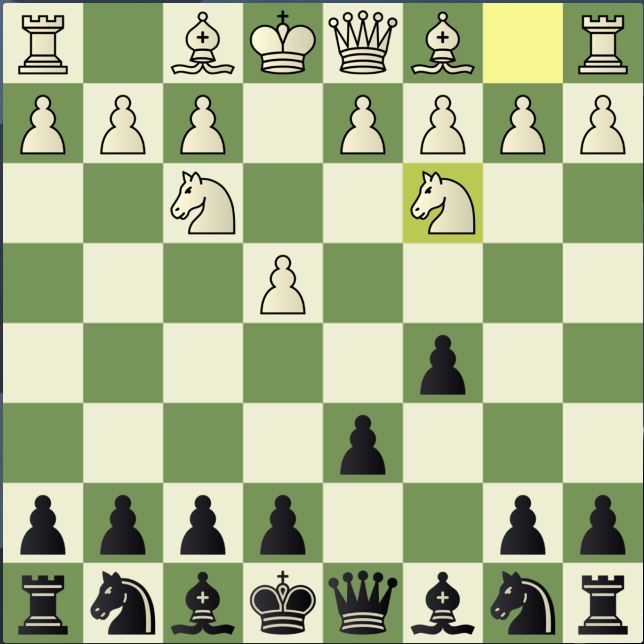
\includegraphics[width=\textwidth]{Images/Design/d-4.png}
            \caption{Siciliana}
        \end{subfigure}
        \caption{Defensas comunes en ajedrez.}
    \end{figure*}
    
    \newpage 
\section{Diagrama de flujo}

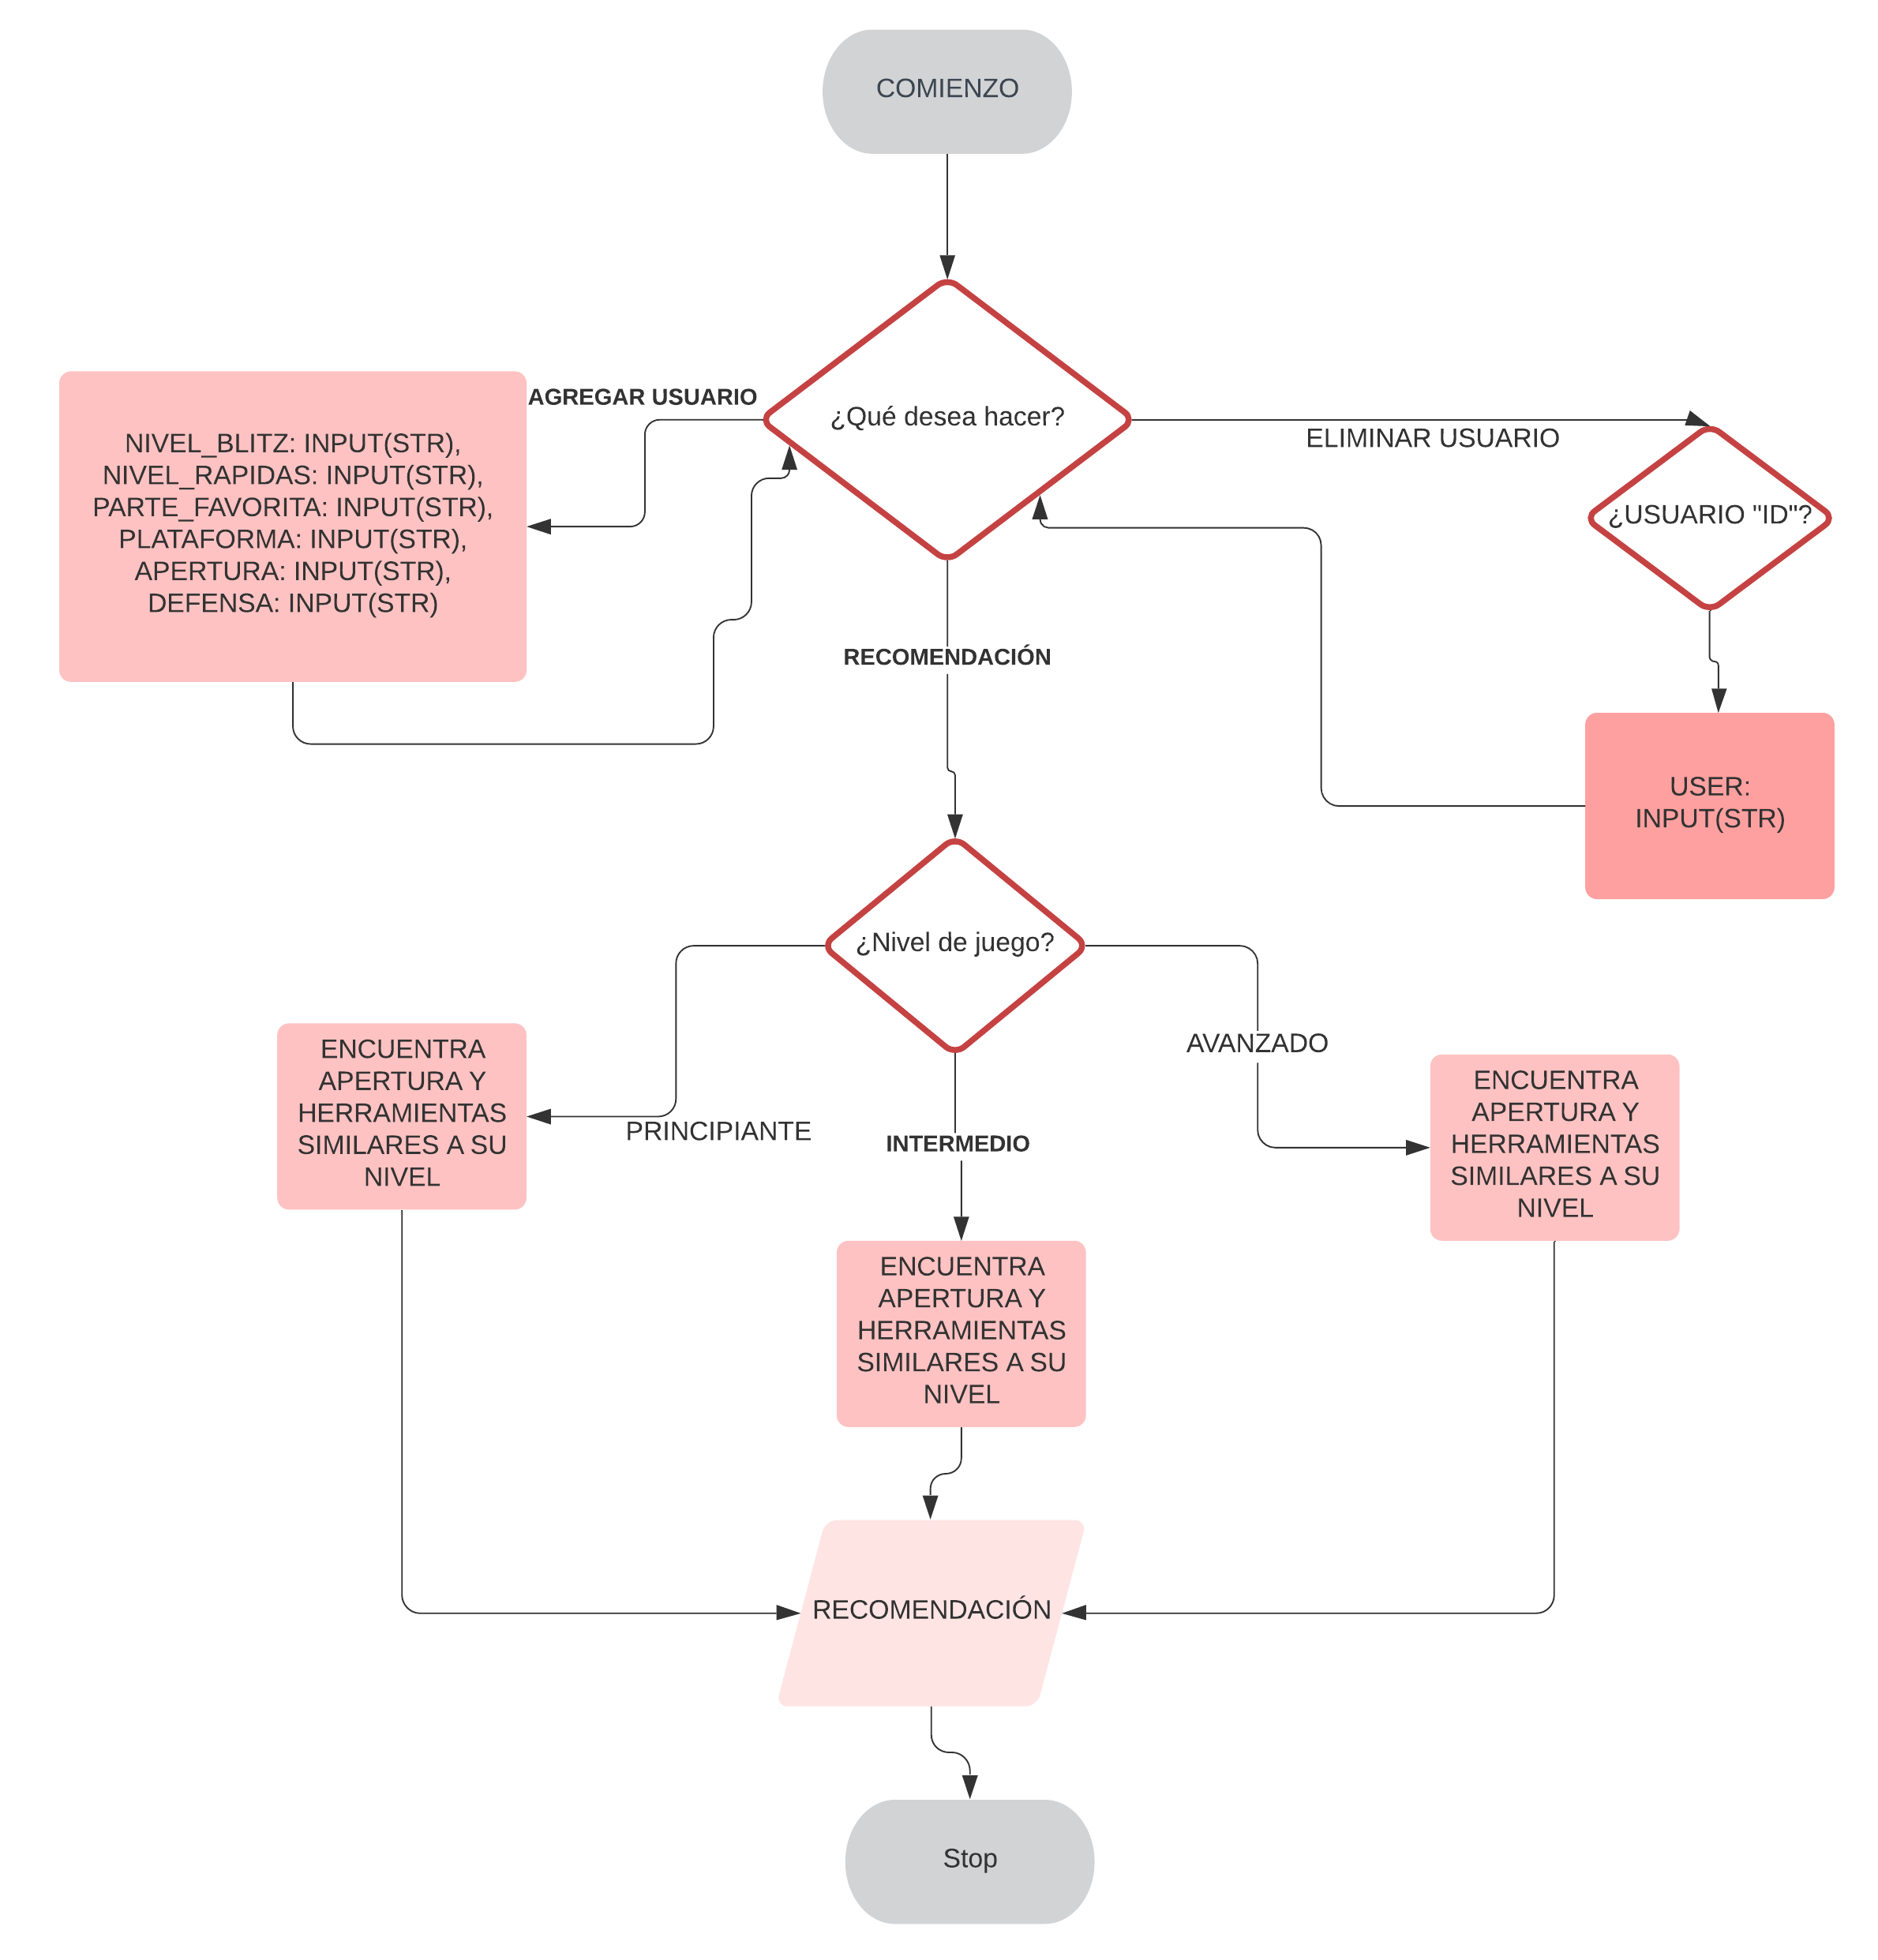
\includegraphics[scale=0.8]{Images/Algorithm flowchart example.png}
\section{Diseño de la base de datos}
Un resumen de la base de datos original obtenida es la presentada en la parte inferior. Su implementación se basa en relacionarla con grafos. El propósito: 

\begin{itemize}
    \item \textbf{Nodos} - Los valores de las columnas.
    \item \textbf{Relaciones} - Los títulos de las columnas, exceptuando «USER». 
\end{itemize}
\begin{table}[ht]
\resizebox{\columnwidth}{!}{%
\begin{tabular}{@{}lllllll@{}}
\toprule
USER    & NIVEL\_BLITZ & NIVEL\_RAPIDAS & PARTE\_FAVORITA & PLATAFORMA  & APERTURA          & DEFENSA   \\ \midrule
user001 & Principiante & Intermedio     & Intermedio      & Chess.com   & Inglesa           & Siciliana \\
user002 & Principiante & Principiante   & Final           & Chess.com   & Fianchetto        & Siciliana \\
user003 & Principiante & Principiante   & Final           & Chess.com   & Italiana/Española & Francesa  \\
user004 & Principiante & Principiante   & Final           & Chess.com   & Italiana/Española & Francesa  \\
user005 & Principiante & Principiante   & Intermedio      & Chess.com   & Italiana/Española & Francesa  \\
user006 & Principiante & Principiante   & Intermedio      & Chess.com   & Italiana/Española & Eslava    \\
user007 & Avanzado     & Avanzado       & Intermedio      & Chess.com   & Sistema Londres   & Caro-Kann \\
user008 & Principiante & Principiante   & Final           & Lichess.org & Fianchetto        & Caro-Kann \\
user009 & Intermedio   & Intermedio     & Apertura        & Chess.com   & Italiana/Española & Siciliana \\
user010 & Principiante & Principiante   & Final           & Chess.com   & Italiana/Española & Francesa  \\ \bottomrule
\end{tabular}%
}
\end{table}

\section{Repositorio}

El repositorio del proyecto se encuentra en el siguiente link:\newline 
\textcolor{blue}{\href{https://github.com/RudiksChess/Grafos}{https://github.com/RudiksChess/Grafos}}




%---------------------------
\bibliographystyle{apalike}
\bibliography{sample.bib}

\end{document}